\documentclass[11pt]{article}
\usepackage{graphicx}
\usepackage{geometry}
\geometry{
 a4paper,
 total={170mm,257mm},
 left=20mm,
 top=20mm,
 }
\graphicspath{ {images/} }

\begin{document}

\title{%
 Agile TweetViz from team Geek!O\\
\large Project Report}
\author{Harsha Kadekar\\
  Yash Chopra\\
  Gowtham Nayak\\
  Anoop Jatavallabha\\
  Seema Suresh}
\date{\today}
\maketitle
\newpage
\tableofcontents
\newpage
\listoffigures
\newpage


\section{Introduction}
The popularity of social media has made twitter an important platform for information transfer, news reporting and public opinion. Despite the significant potential for measuring public opinion, finding the perspective for any topic by sorting through massive number of tweets is an arduous task. To counteract this problem, our vision is to give tweet visualization a new meaning by distinguishing and filtering out tweets that are of concern to the user. This meaning can be derived in a top-down tree like format so that the bottom most node per say, gives the detailed view on a topic, be it social/technical. The idea is to look for keywords that matches best from the given statement and jolt it down further to extract popular users (with tweets that mattered the most to other users) and hashtags that are relevant. Further, these popular people profile and hashtags are combined to obtain a single visualization that gives an overall popularity and analysis of the topics of interest.

 The tweets are fetched based on user given topics, where topics can be anything from a word to few sentences. This process is achieved by using two separate libraries in Python: NLTK library (Natural Language Toolkit) and Tweepy library. For analyzing tweets, a smalltalk based platform Moose/Pharo is used where a metamodel is defined which in turn will feed data for visualization. Finally, visualization is achieved using Roassal library in Pharo.
 
We have demonstrated assorted visualization, trying to utilize the maximum power of Roassal library, while establishing relationship between different aspects of tweet and its user. 

\section{Filtering and sorting of tweets based on hashtags, user and tweet relationship}

Twitter is a platform, where individuals can express their views by using sentences having 140 characters or less. These tweets can further be liked or retweeted by other followers, thus increasing the area of viewership among the users of Twitter. Another important characteristics of Twitter is the association of tweets with a certain topic by using "hashtags". A hashtag is created by placing a "\#" in front of a word. By doing so, a tweet can be tagged to a certain topic. A tweet can have a single or multiple hashtags thus representing either one or multiple topics simultaneously. For example, to express a security concern in Java, a tweet can be mentioned as "A prog example of trojan using Java. Be aware of threat! \#java \#security" or to announce a job posting a tweet can be mentioned as "Experienced software engineers needed for front end development. DM me details. \#java \#UIdesign \#jobs". By mentioning more than one hashtag in a tweet, a user is trying to establish the relationship between two different topics. Therefore, in our second example, we can find same tweet by searching \#java and \#jobs. Hashtag relationship is important because using this on a single tweet level, we can establish a tweets relationship to various topics. But on massive level we can find the pattern of user and tweet to vast majority of social/technical topics. The added advantage is, as security was the most used hashtag, our program will make sure that we include the tweets that are concerned with the security of software only. It will keep the focus directed towards the main topic and will not wander off and start considering the other security based topics such as national security, community security, etc.

We are grouping the tweets into this hashtag relationships with a common root hashtag. Apart from this we are trying to build the relationship between number of tweets a user tweeted about a topic. Finally combining the popularity of a hashtag and user and grouping all those tweets which falls under both these group to get the most relevant tweets.

\section{Requirements: Problem Statement and Specifications}
We have gathered our initial requirements from SCORE website\cite{SCOREwebsite} and have further refined them by conducting brainstorming sessions with the team and online meetings with our project sponsor.

We have developed different user stories which would help us to achieve our vision of the project. 

\begin{itemize}
\item Our one of the part of vision was to fetch meaningful tweets based on the user input. To achieve this we had "USER-STORY52:As a user of Tweet Viz, I should be able to give the topic or sentence to the Product, using that topic/sentence product has to fetch tweets"

\item Second important part of the vision was to analyze fetched tweets in a meaningful way. To achieve this we had "USER-STORY53:As a developer I need meta models to store the tweets, user details, hashtags, location etc. in objects. These objects will be used to carry out visualization." or "USER-STORY23:As a user, I would like to relate the fetched tweets with their user handles"

\item Third important part of the vision was to visualize the way which can clearly show the grouping of tweets and users, hashtag popularity, hashtag relationships. To achieve aspects we had different users stories like - "USER-STORY95:As a user I would like a graph representation of the retweets and favorites for each hashtags", "USER-STORY24: As a user, I would like to visualize tweets with the user who have tweeted them", "USER-STORY79: As a user I need to get a visualization pattern based on the given search category"

\end{itemize}

Apart from this we had certain process requirements like

\begin{itemize}
\item "USER-STORY25: Pharo/MOOSE has to be used for analysis of tweets"
\item "USER-STORY26: Roassal should be used for visualization of analysis done on tweets."
\end{itemize}

We have achieved our vision by first establishing the flow of hashtags and further relating those hashtags to the twitter users and their tweets. Secondly, we have utilized this relationship to categorize the tweets and tweet handlers into different groups. Finally, we have visualized the analyzed tweets and their relationship so as, this relationship can be observed and studied in a much compact and simpler manner.
This analysis will help us to determine the popularity of an user in a particular field of interest. For example, user is tweeting on the topics related to \#Java, \#Security, \#Job, \#Issue, and \#JDK. Among these topics, \#Security is the most popular hashtag. This condition can be determined based on the counts of retweets and number of likes on a tweet. Our aim is to clearly understand user area of expertise. In this case, it is Java Security even though user is tweeting about issues, job and jdk.


\section{Development Process}

In this project we used Agile methodology with Scrum process. The main reason to choose was for its ability to produce deliverable from beginning even without having full set of clear requirements. For example, we were sure on how to proceed for the user stories related to Tweet fetch, but were unclear on the methods that will be used to create meta-model and visualization. Considering this, agile lets us start working on the known components from the day one. Another reason to choose Scrum was for its ability to handle changes effectively. It provided us the capacity to continuously update the backlog, while refining requirements in the background and at the same time working on known components of the project. In the beginning of project our understanding of requirements was only limited to what was mentioned on SCORE website. We knew this will change after our meeting with our sponsor and so it did. Scrum ensured the risk involved with the updating requirements and using new and unknown tool have minimum negative impact on our project. 

From risk management perspective, we were able to identify two major hurdles that we may face during the project duration: 

\begin{enumerate}
\item Lack of knowledge of Pharo/MOOSE may slow down this time sensitive project.
\item Whether chosen Database Management System would handle or scale to the fetched twitter payload.
\end{enumerate}


Lack of understanding of Pharo/MOOSE was our biggest challenge. We dedicated one full sprint out of 5, trying to get better understanding of the new language and environment. We were skeptical about the "What if not" part of the learning process, thus discussing number of other options. First option discussed was; can the functionality depending on the PHARO/MOOSE be developed using some other technology? We identified that these functionalities can be implemented to some extent using the libraries provided by the python and also javascript, but the unique feature of Pharo/MOOSE is object profiling. The features of MOOSE/PHARO help in the easy creation and integration of meta model and visualization as both are closely related. Given that, use of Pharo/ Moose was also part of process requirements, moving out of Pharo/MOOSE was ruled out. To improve the technical knowledge each team member was given certain topics in the Pharo/MOOSE in parallel to the product development. Thus filling the knowledge void.

Secondly, we were not sure what should be the preferred data storage method as we were planning to store 1 million tweets. Our initial choice of Database was Microsoft SQL Server Express edition. After doing the feasibility study of space and time impact of million tweets database interaction, it was found that Express edition was not able to handle 1 million records due to storage restriction. We decided to go ahead with MySQL. But the question that followed was whether or not we need to use Database at all in the project. As we were fairly new to MOOSE, we were not sure of configuring and accessing database from MOOSE. After further reading and research, we got a better way of adding packages that could directly read from CSV file. This helped us to easily create the meta-model for the project. After exploring and discussing all the options mentioned above, we were clear of right solution, thus making rest of the project development a smooth sail.  

As both the platforms were new to us, the main task in our first sprint was to understand them. We went ahead and generated our first set of product related user stories. Some of the user stories were vague, we discussed this problem with our sponsor Dr Alexander Bergel, Dr. Kevin Gary and later conducted brainstorming sessions to create better user stories. We decided to place more emphasis on Meta-model creation and visualization, rather than user interface. 

Agile helped us to continuously add or change the requirements without hindering the product development. At the end of first sprint, requirements related to fetching of tweets were finalized while, still debating on meta-model and visualization. Requirements for Meta-model and Visualization were finalized at the end of sprint 2 and sprint 3 respectively. We discussed with the sponsor after the 4th sprint and then incorporated the changes to the existing requirements. Any unclear requirement acted as a placeholder for a conversation with the product owner to better understand the requirement. Software Requirements Specification(SRS) were updated throughout all the sprints.

Taiga and Google site were used for implementation of software process whereas Git was used for change management.


\section{Architecture and Design}
From the technical aspect of the project description, it was clear that 3 main parts of the project are

\begin{itemize}
\item Creation of meta model
\item Visualizing the tweets present in the meta model
\item Finally answering some questions from that visualization and analysis.
\end{itemize}


Based on the present information, it was deducted that we need a separate module for the meta-model creation. Our code should have the ability to analyze the tweets and generate the meta-model thus establishing the relationships between tweets. Once we have the meta-model, based on the 2nd technical requirement we have to visualize different components of tweets. Different components of tweet from same meta-model can be used in several forms to create various visualizations depicting different meaning. For addressing all the 3 points, it is very important to have meaningful set of tweets. Fetching tweets doesn't come under meta model creation or visualization modules. We need a separate module which has the ability to fetch meaningful set of tweets from twitter and can pass it to meta model module more like a business logic layer. That's why we have come up with the following 3 different modules for our product.
\begin{enumerate}
\item Tweet Fetch - Get meaningful tweets
\item Tweet Analysis - Create meta-model
\item Tweet Visualization - Visualize the relationship of tweets.
\end{enumerate}

\begin{figure}[h]
\centering
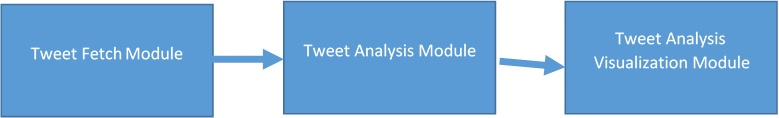
\includegraphics[width=\textwidth]{HighLevelDesign.jpg}
\caption{High Level Modules}
\end{figure}

\subsection{Tweet Fetch}
Tweet fetch Module is responsible for fetching tweets based on user input. This module can further be divided into three main parts: 
\begin{itemize}
\item Processing user input
\item Fetching tweets
\item Storing tweets.
\end{itemize}

A user input can be anything from a single word to a complete sentence , which is then parsed to generate hashtags. These hashtags are used to search and download the relevant tweets. Once the tweets are downloaded, they are stored in SQL table and CSV file. Our next module, Tweet Analysis, directly takes CSV file as input. 
DataStorageReader as outlined in figure 2, is responsible for reading configuration file, interacting with TweetViz MySQL DB and interacting with CSV file through filereaderwriter component. Configuration file contains following parameters - SQL connection related parameters, Type of tweets fetched - most recent, popular, mixed; Type of storage - CSV or SQL, CSV file path, Debug level
 
For security reasons, Sql parameters are encrypted and stored in configuration file. HashtagGenerator is responsible for generating the hashtags from the given user input using natural language processing. TweetFetch component will get the tweets from Twitter based on the given hashtags. TweetBackend is responsible for the integration of all the different components. 

During the design of modules we have incorporated many design patterns.
\begin{itemize}
\item Interaction between HashTagGenerator and DataStorageReader is a better example of Observer pattern. $Tweet_Fetch$ module first calls the HashTagGenerator to generate hashtags and fetch the tweets related to those generated hashtag. Once this event is complete, it calls the DataStorageReader to store those generated tweets. Also we intended to use Observer pattern for interacting with the web interface. But it was not taken up due to priority given by sponsor.
\item We made DataStorageReader class a singleton. We wanted a single point of communication for the database. All the different sub modules of $Tweet_Fetch$ should interact with database via a single object of DataStorageReader. By this we are avoiding multiple connections to the database as well.
\item DataStorageReader class is a single interface for any communication regarding storage and reading of the data. This storage and reading can be done in two ways – Database or CSV. So DataStorageReader provides functionality to write/read to database and similarly write/read to csv file. But actual csv read and write is done by CSVFileReader. So DataStorageReder will pass on the information to CSVFileReader which will do the actual csv file writing and reading. Here we tried to incorporate Adapter pattern.
\end{itemize} 


\begin{figure}[h]
\centering
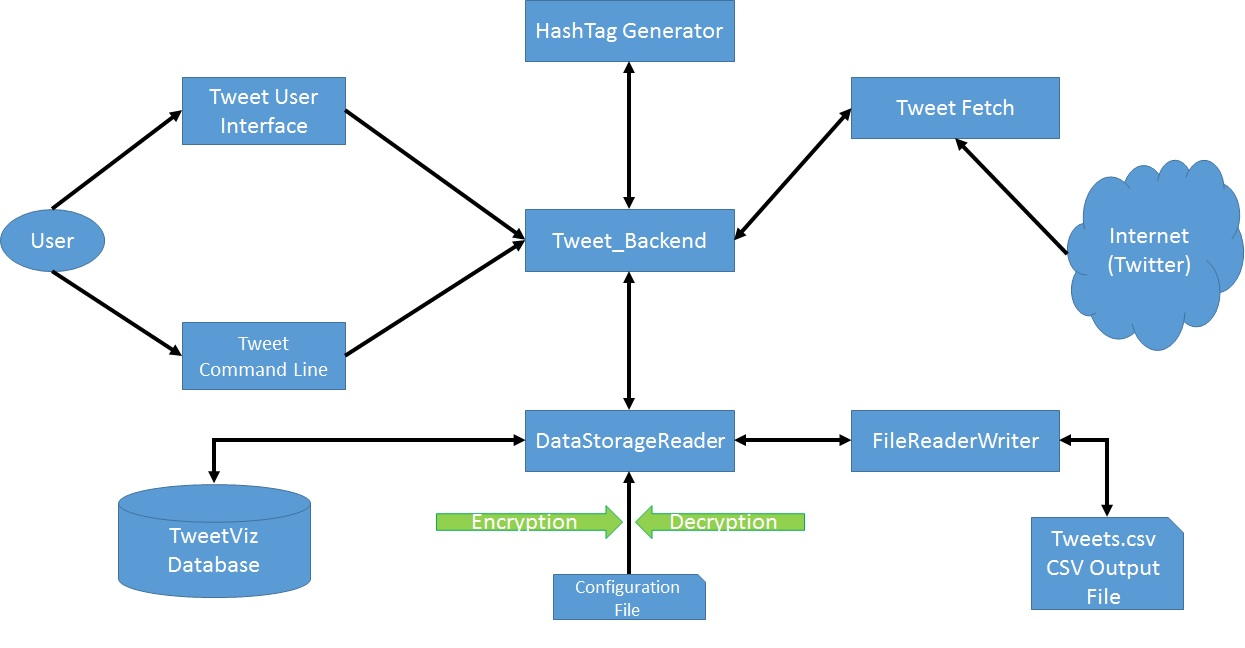
\includegraphics[width=\textwidth]{TweetFetch.jpg}
\caption{High Level Design of Tweet Fetch Module}
\end{figure}


\subsection{Tweet Analysis}
Two main responsibilities of this module are: Read the tweets and Generate the metamodel. CSVFileToTweetVizModel as outlined in figure 3, will use Neo-CSV package of MOOSE to read the CSV file and further generate the metamodel. Metamodel has inter-related objects representing Tweet, Tweet-User, HashTag and SearchCategory. 


\begin{figure}[h]
\centering
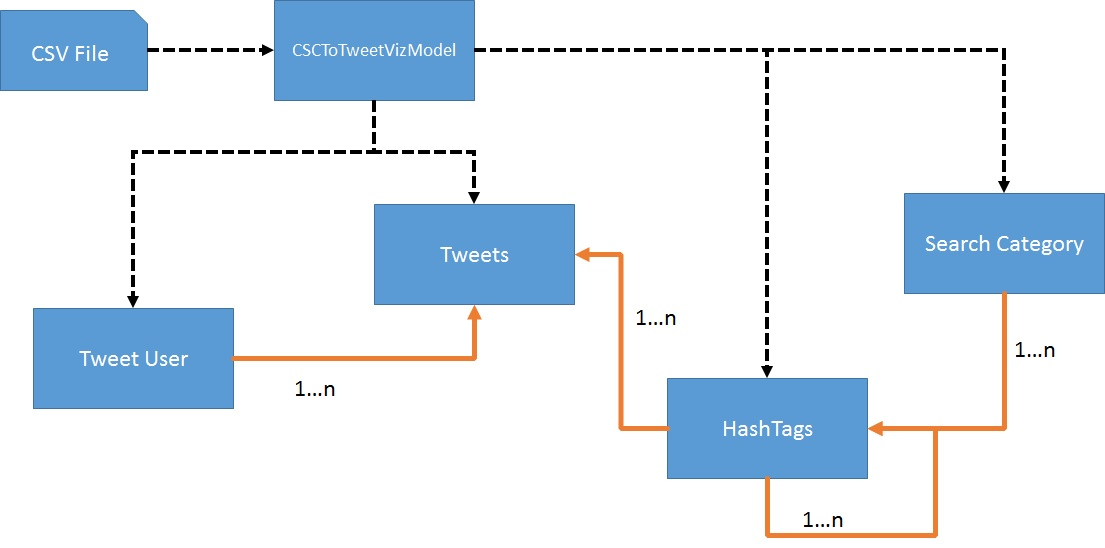
\includegraphics[width=\textwidth, height=5cm]{TweetAnalysis.jpg}
\caption{High Level Design of Tweet Analysis}
\end{figure}

\subsection{Tweet Visualization}
Multiple visualizations are generated representing the relationships between different objects of the metamodel. To achieve this, we have used RTView and Roassal package in Pharo/MOOSE. 


\section{Project Plan}
Project development was divided into five iterations. First sprint was utilized for understanding of requirements and analysis of tools; next 3 sprints were dedicated for development of the major technical components of product; and last sprint was allocated for integration, testing and documentation. Sprint meeting was conducted on every alternate Saturday (end of every sprint), where sprint agendas were discussed/ demonstrated. Major milestones of the project can be described as - 
\begin{enumerate}
\item Sprint 1 (21 SEP 2015-04 OCT 2015): Understanding tools and requirements
\begin{itemize}
\item Demonstrate different tools mentioned in requirements as learned by team members. 
\item Participate in brainstorming session to further elaborate the requirements of the project. 
\end{itemize}

\item Sprint 2 (05 OCT 2015-18 OCT 2015): Obtain user input in the form of a word or a sentence.
\begin{itemize}
\item Parse the user sentence to build hashtags.
\item Fetch the tweets based on hashtags.
\item Store the fetched tweets
\end{itemize}
After this sprint, the demo was presented in front of an external reviewer, Dr. Kevin Gary and his inputs were used to make technical and procedural changes to our project.

\item  Sprint 3 (19 OCT 2015-01 NOV 2015): Analysis of tweets
\begin{itemize}
\item Analyze the data to produce Tweet objects in MOOSE
\item Analyze the data to produce Hashtag objects in Pharo
\item Analyze the data to produce User (Twitter handles) objects in Pharo.
\item Analyze the data to produce Search Category (Application user input) objects in Pharo
\end{itemize}
The working model will demonstrate meta-model containing several objects. These objects will be further used in Roassal library for the visualization thus offering user the opportunity to review the topics of visualization.

\item Sprint 4 (02 NOV 2015-15 NOV 2015): Visualization of meta-model
\begin{itemize}
\item Visualize Hashtag tree relationship. 

\item Visualize Hashtag and Tweet words cloud relationship. 

\item Visualize User, Tweet and hashtag organization chart relationship. 

\item Visualize User and Tweet connection circle relationship. 

\item Visualize tweet messages of different tweets. 
\end{itemize}
The demo will present different visualization based on generated meta-model. There are several different types of Smart-arts and charts presented to demonstrate the wide range of visualization power of Roassal library in Pharo. 

\item Sprint 5 (16 NOV 2015-23 NOV 2015): Regression
\begin{itemize}
\item Integrate all the modules of the product.
\item Complete documentation related to product and project.
\item Full system run from user input to final visualization.
\end{itemize}
The focus of this sprint was on the integration of separate modules and testing the code in parts and in full. The system needed to perform flawlessly.
\end{enumerate}



\section{Management Plan}
We followed Agile work environment with two weeks of sprint duration and conducted stand-up meetings on every alternate day. For every sprint meeting, the first half was dedicated to sprint review and second half of the meeting was reserved for sprint planning. Sprint review focused on the following points: 
\begin{itemize}
\item Which tasks were left incomplete and the reasons behind them? 
\item What worked well for us?
\item What didn't worked well for us?
\item What actions can we take to improve our process?
\end{itemize}

In the sprint planning, following things were discussed: 
\begin{itemize}
\item Objective of the new sprint.
\item Any new user stories or any change to the priority of the user stories 
in product backlog?
\item  Which users stories needed to be moved from product backlog to sprint backlog? 
\item Allocation of tasks and roles of different team members (tester/developer/product owner)

\end{itemize}
 
Three questions answered by each team member in the daily stand-up meeting were 
\begin{enumerate}
\item What did I do?
\item What I will be doing till next meeting? 
\item Is there any issue which team must know OR Is there any help needed from the team? 
\end{enumerate}

Two tools helped us monitor the whole process - Taiga\cite{TaigaSite} and Google Site\cite{GoogleSite}. Taiga was used as our visual management board that helped us to keep record of the product backlogs(figure 4) and sprint backlogs (figure 3). 

Once the user story has been moved from the product backlog to the sprint backlog, the state of the tasks of user stories can be monitored during that sprint as: New, In progress, Testing or Completed. Each user stories were provided with unique ID for traceability and a point (5, 10, 15) based system for prioritization. User stories or tasks were also provided with a unit test/ developer integration test (figure 6). 

For any task that did not involve coding, a knowledge base document was written to explain the final outcome of the task. For example, our first sprint mostly consisted of the tasks that involved learning new platforms like MOOSE, PHARO, etc. In this case, a document was prepared explaining the concepts learned and shared with the team. Issues were logged in the Taiga’s issue tracker tool. 

Google site\cite{GoogleSite} was a bird eye view of what was going on in the team. Every sprint and stand-up meeting details were recorded, including date of the meeting and important points discussed. Documents related to the process and product were placed in the wiki section of the site. 

\begin{figure}[!ht]
\centering
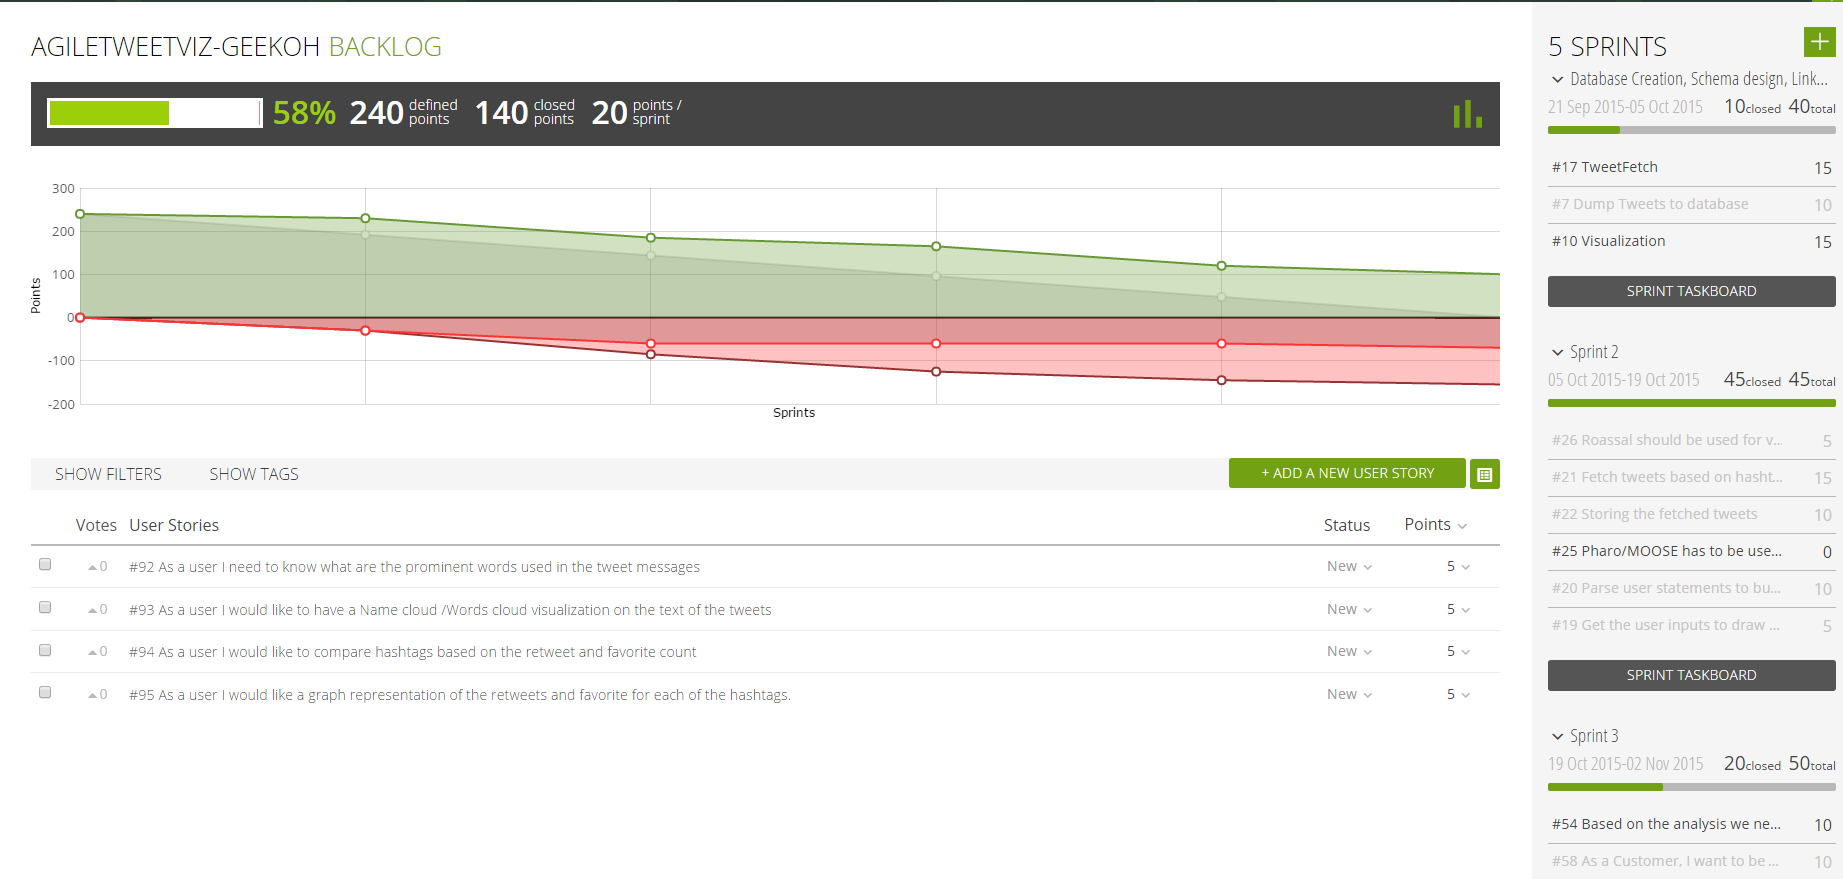
\includegraphics[height=11cm]{Backlog.png}
\caption{Product backlogs in Taiga\cite{TaigaSite}}
\end{figure}

\begin{figure}[!ht]
\centering
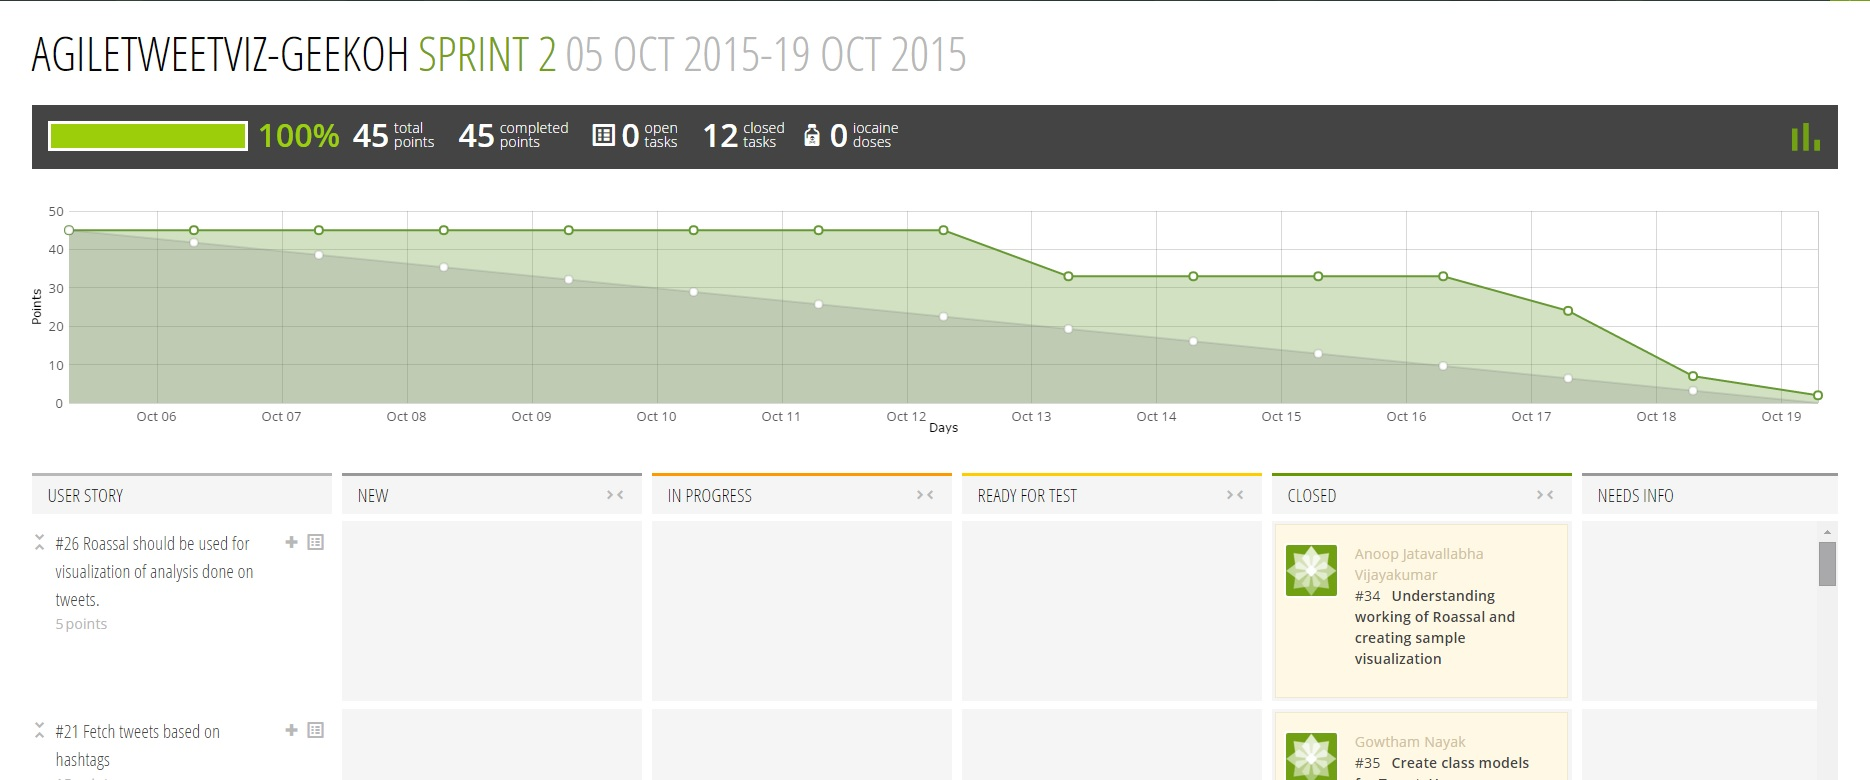
\includegraphics[height=11cm]{SprintBoard.jpg}
\caption{Virtual Sprint Board in Taiga\cite{TaigaSite}}
\end{figure}

There were two scheduled reviews for Quality Assurance. These reviews were performed by Dr. Kevin Gary after sprint 2 and sprint 5. The feedback after first review were: 1) User stories are not formed correctly - This should be the place holder for the conversation with the customer. 2) Many of the tasks were being closed nearing the end of the sprint. Both of these points were taken into account and further improved on. 


\begin{figure}[!ht]
\centering
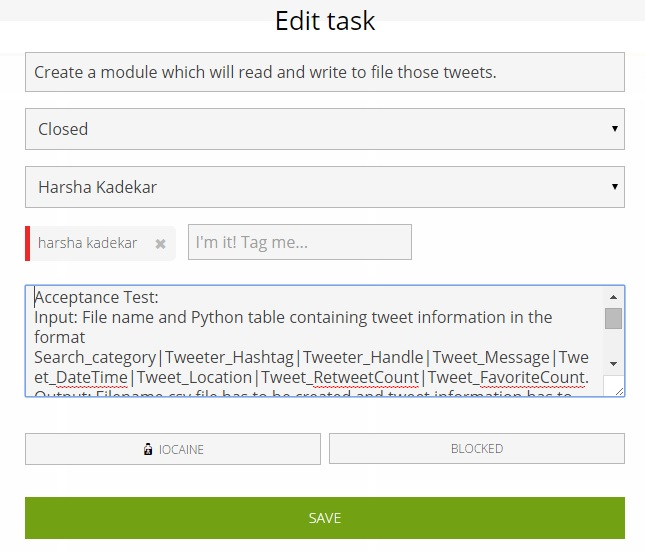
\includegraphics[width=10cm, height=10cm]{TaskInfo.jpg}
\caption{Task information in Taiga\cite{TaigaSite} }
\end{figure}


\section{Implementation}
As mentioned in the architecture, there are three main modules in this product.
\begin{itemize}
\item Tweet Fetch
\item Tweet Analysis
\item Tweet Visualization
\end{itemize}

Tweet Fetch module (Figure 7) was completely developed using python. Various packages used for implementation are:
\begin{itemize}
\item Tweepy - Fetch tweets from Twitter.
\item Mysql Connector - Interact with MySQL database.
\item NLTK - For natural language processing of user input.
\item Py2Exe - To convert the python scripts to a deliverable.
\end{itemize}

Best coding practices including naming conventions for variables, functions, files and folders, comments and logging were discussed and followed throughout the project. All the commits to the Git were accompanied by the taskid and a brief explanation of the changes made to the code.

\begin{figure}[h]
\centering
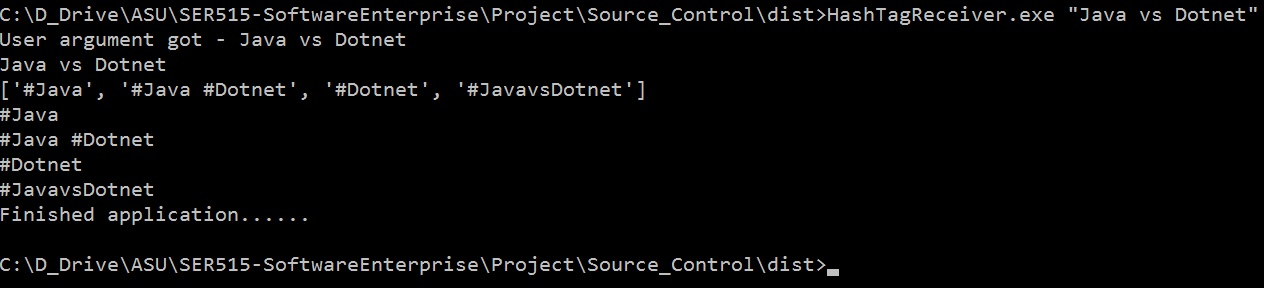
\includegraphics[width=\textwidth]{TweetFetchImp.jpg}
\caption{Tweet Fetch module execution}
\end{figure}

Tweet Analysis and Tweet Fetch modules were developed in SmallTalk based Pharo platform. Pharo and MOOSE has inbuilt source control. All the packages created in the "package-cache" folder of MOOSE were also checked into Git with proper comments.

Visualizations developed during the course of our implementation are

\begin{enumerate}
\item Given a set of tweets based on a search category, we are able to get the hashtag's relationship. This is an important part of the vision. Here we are developing a tree like relationship of hashtags and finally identifying important hashtags relating to the input provided by user. Initial aqua color ellipse in the figure 8, is user input whereas purple ellipses are the hashtags generated from the user input and red color boxes represent the next level of hashtags.
\begin{figure}[h]
\centering
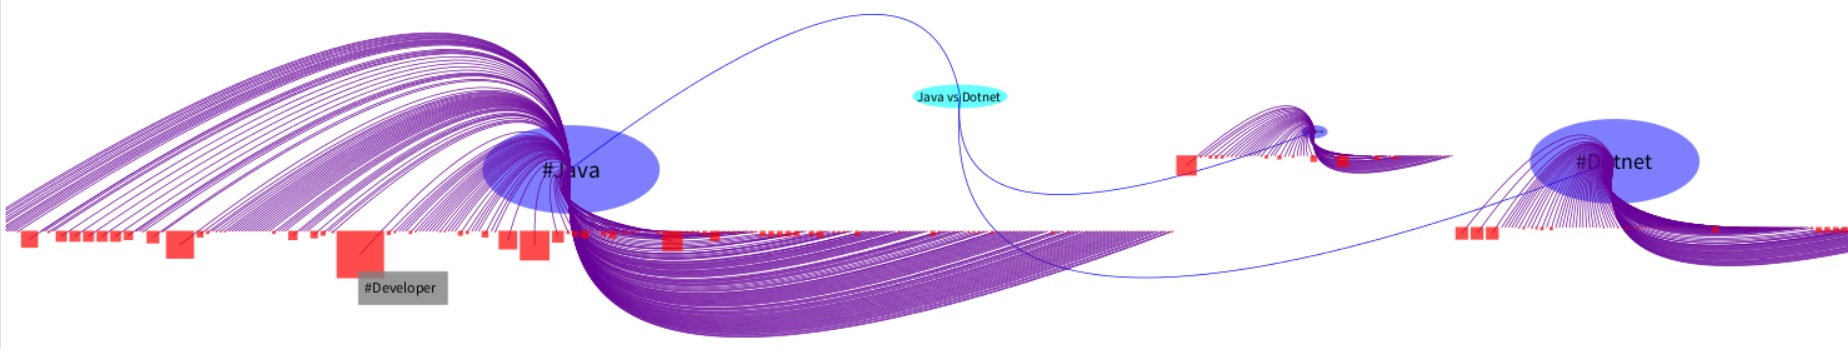
\includegraphics[width=\textwidth, height=8cm]{JustHashTags.jpg}
\caption{Hashtag relationship}
\end{figure}
\item Once the hashtag's relationship has been generated, the tweets were added in the visualization. In this visualization we are trying to group the tweets into different hashtags. As we identified the prominent hashtags, by associating the tweets to them are trying to identify those tweets which are more relevant. In figure 9, green color ellipses in the outer circumference represents the tweets. Blue color ellipse is the main hashtag whereas red color boxes are sub hashtags. Size of the red color boxes depends on the number of tweets associated with that hashtag.

\begin{figure}[h]
\centering
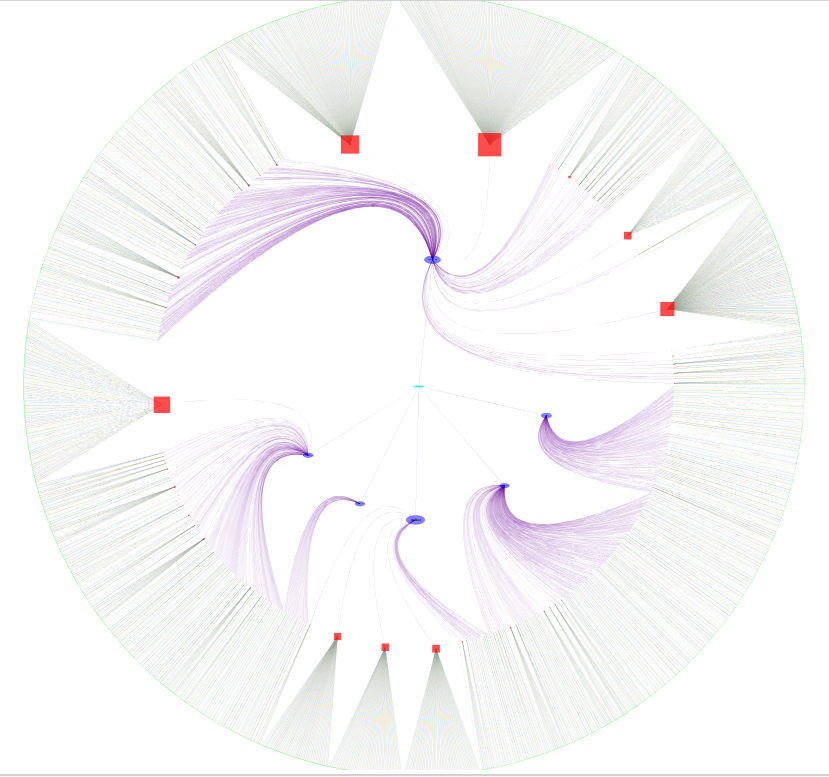
\includegraphics[width=10cm, height=10cm]{HashtagToTweets.png}
\caption{Tweet - hashtag relation}
\end{figure}

\item In figure 10, we have generated visualization based on users and their tweets. Here idea is to identify most popular users who have more tweets related to the given user topic. Here purple ellipses are users and red color boxes are tweets. Size of ellipse is dependent on the number of tweets by that user. Initially, users and tweets are displayed separately. Once the "connect" Button clicked(figure 11), all the tweets tweeted by a user will come together and circle around that user.
\begin{figure}
\centering
\begin{minipage}{.5\textwidth}
\centering
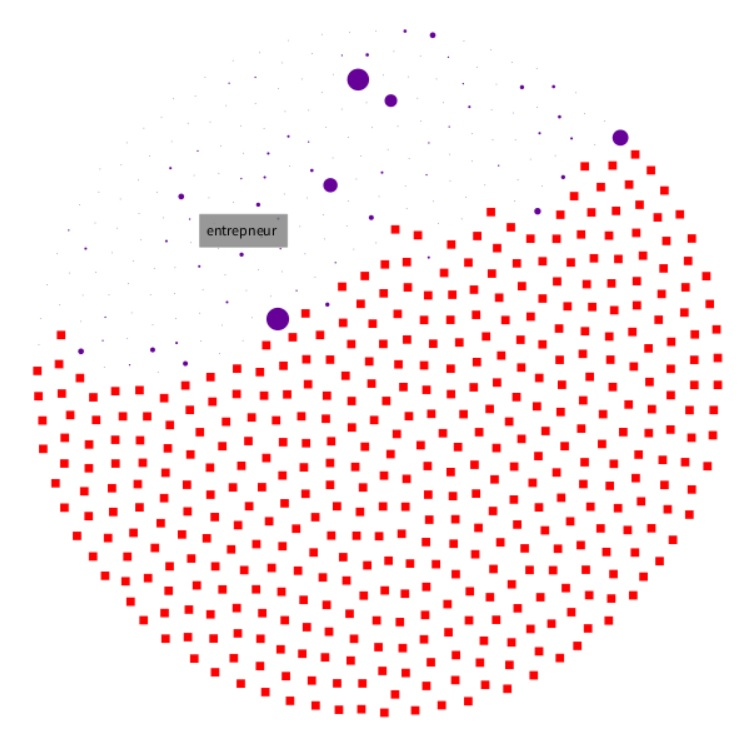
\includegraphics[width=.8\linewidth]{UserTweet1.jpg}
  \caption{User and tweets}
\end{minipage}%
\begin{minipage}{.5\textwidth}
\centering
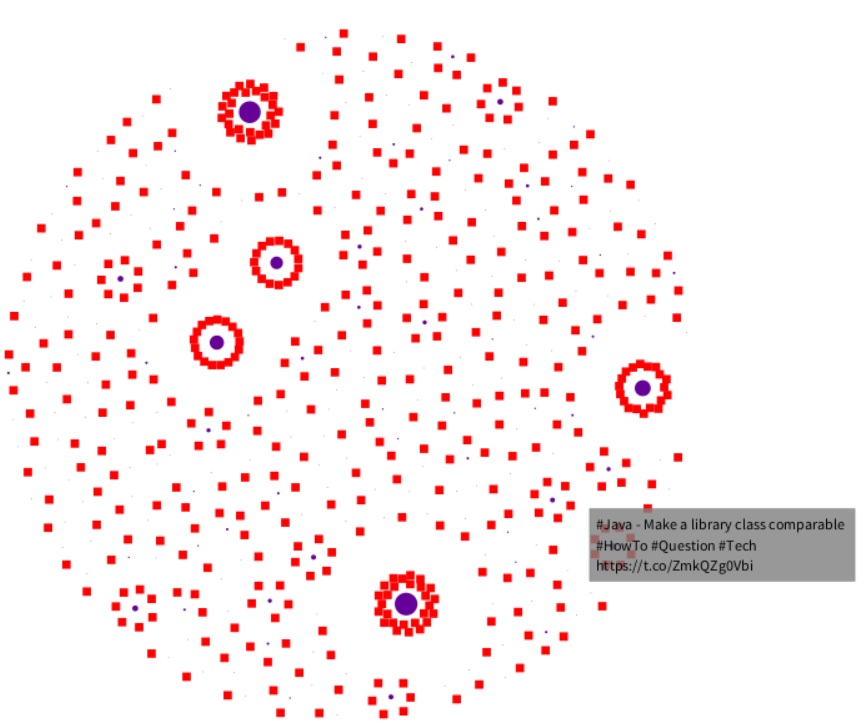
\includegraphics[width=.8\linewidth]{UserTweet2.jpg}
  \caption{Connected User and tweets}
\end{minipage}
\end{figure}

\item Popularity of a hashtag in terms of simple graphs(Figure 12). This gives simple understanding of which hashtags are popular based on the tweets associated under that hashtags.
\begin{figure}[h]
\centering
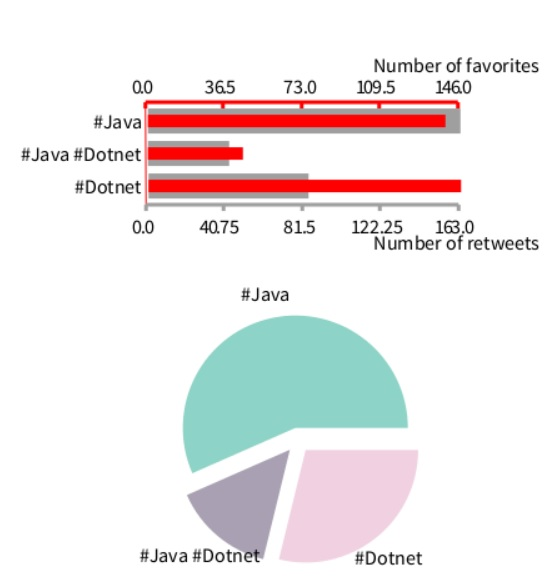
\includegraphics[width=8cm, height=8cm]{Graph.jpg}
\caption{Popularity of tweets}
\end{figure}


\end{enumerate}

\section{Validation and Verification}
We have put more emphasis on verification then validation, which in future we would like to change and give equal importance to the validation part of the project. As part of verification we had unit test cases, developer and system integration test cases and finally regression test cases. As part of validation we had acceptance test cases. Validation was performed by manual inspection were visual patterns were matched to the speculated results of small number of tweets. To specify some, we visited the tweeter's profile to check if he/she is actually relatively influential by analyzing retweet for his/her other tweets. Similar approach was followed for validating popularity of hashtags.

Further for validation, we have created a survey, where participants were chosen randomly, making sure no one was the stakeholder of the project. We have evaluated the responses from 20 participants as our initial validation process. Survey was conducted for Figure 8, Figure 9 and Figure 11; asking participants 1)The level of understanding of the visualization, 2) Can they identify the most prominent part of the visualization 3) How can we change the visualization to be more intuitive. The results relating to Figure 8 indicated that nearly 50\% of the users found it difficult to interpret the visualization. One of the reason is the disassociation of the visualization to the regular twitter use. Visualization of Figure 8 presented the flow of hashtags which did not directly relate to how twitter is used by an individual. This visualization was important for the project, as it was building block for our vision and led to more advanced visualizations as we progressed in the project.

The second visualization(Figure 9), which depicts a direct relationship between the hashtag and tweets showed a more positive understanding among the users. The reason for more positive response was the different layers in visualization, more color coding and the lines connecting between layers were not intersecting. Thus making it easy for the users to understand the figure at first glance.
 
The final visualization(Figure 10 and Figure 11) displayed the most positive result among the three visualizations. More than half of the users reported it to be easy(30\%) or very easy(30\%) to grasp. Our hypothesis says that the ease of understanding of Figure 11 is due to to the reason that this was the most relatable visualization from a user point of view. It was the relationship between twitter user and the tweets, which directly coincides with the basic understanding of twitter. 


Taiga\cite{TaigaSite} was the tool used to report and track any issues during the time of product development.

\begin{figure}[h]
\centering
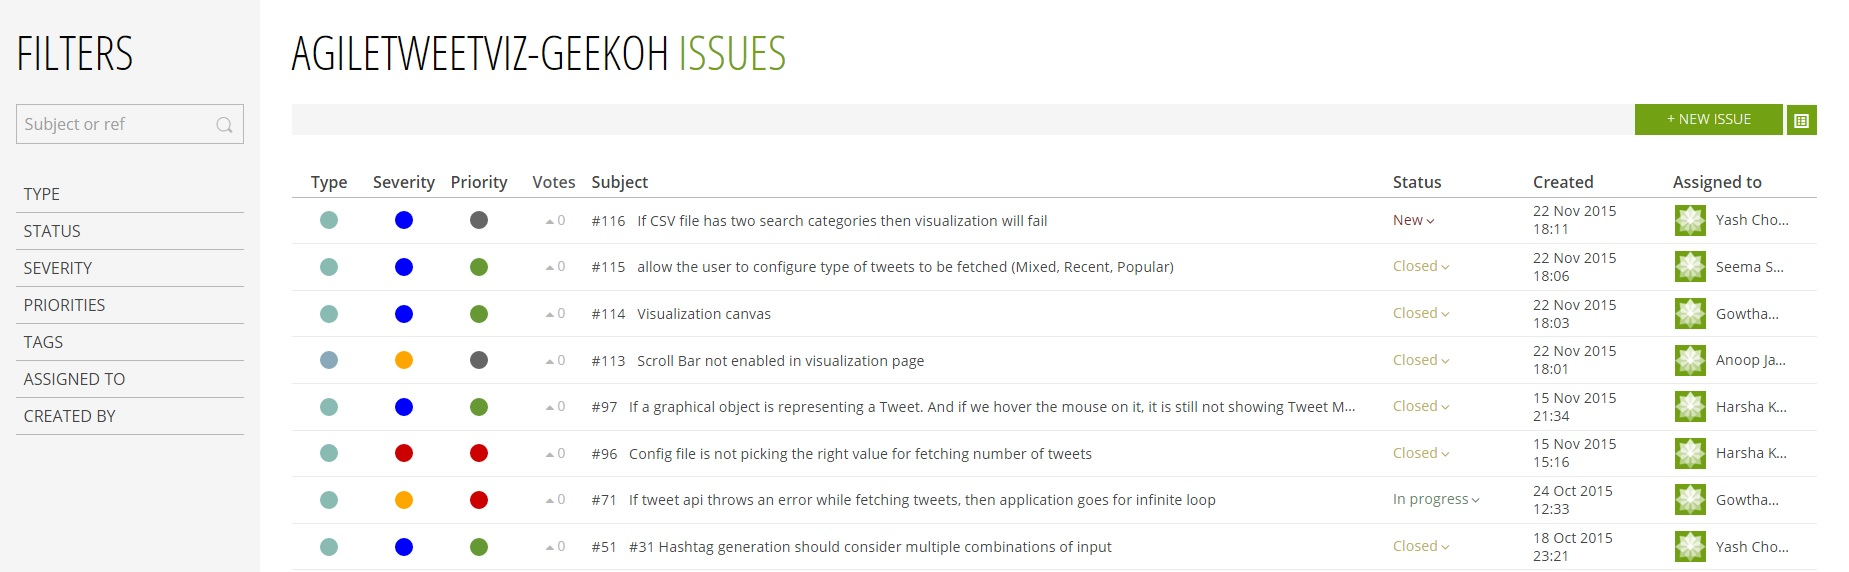
\includegraphics[width=\textwidth]{Issues.jpg}
\caption{Issues list in Taiga\cite{TaigaSite}}
\end{figure}

Every issue when being logged, has to mention the task under which this issue has occurred unless it was discovered during regression or system integration testing. Taiga gives the classification of issues as bug, question or enhancement. Apart from that, priority is provided as low, medium or high. It also classifies the bugs as severity:  minor, normal, important, critical or wish-list. Any issue can be in one of the stages: New, In-progress, Ready for test, Closed, Needs Info, Rejected, Postponed. 

\begin{figure}[h]
\centering
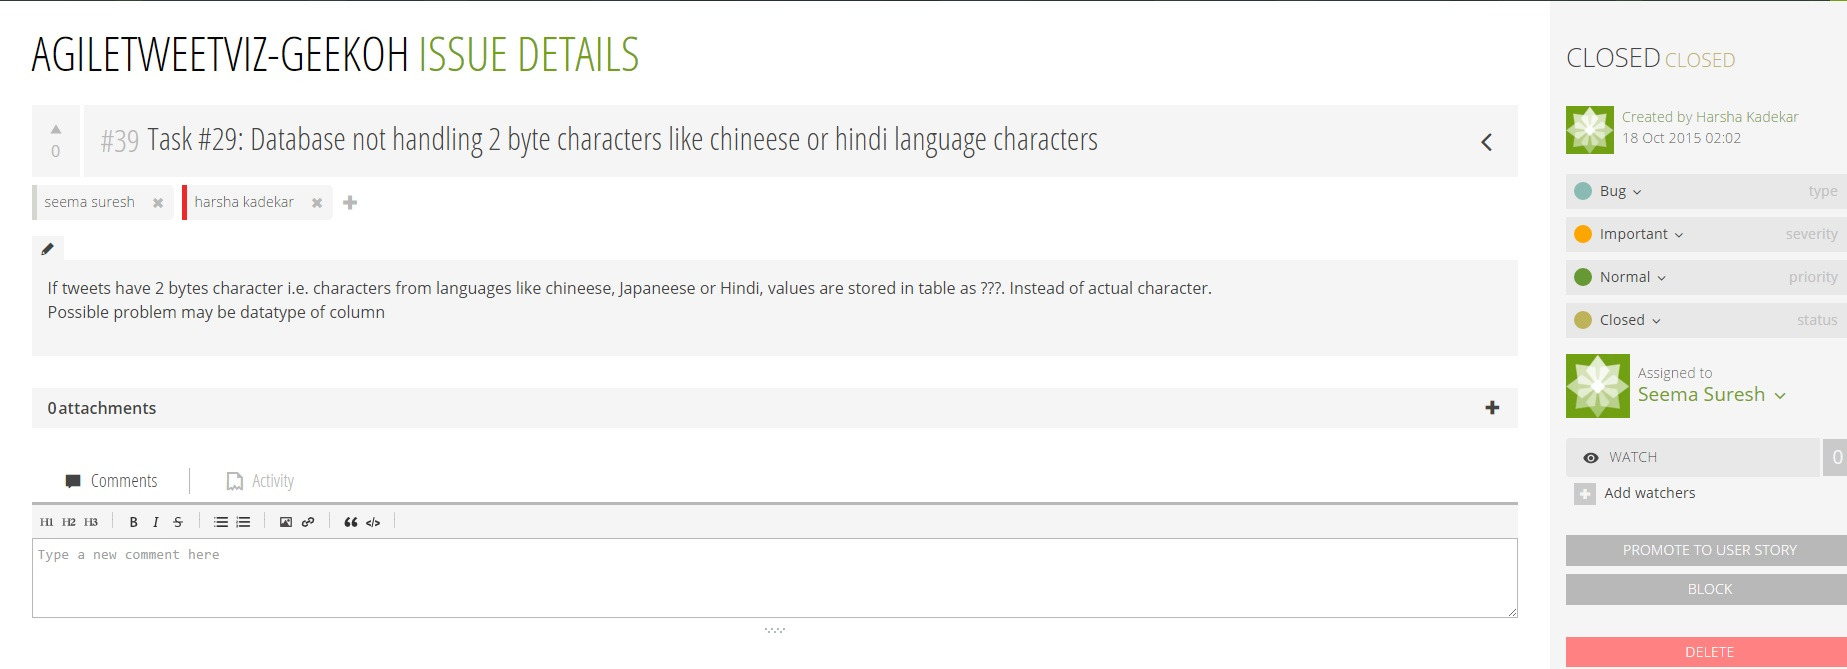
\includegraphics[width=\textwidth]{Issue2.jpg}
\caption{Issue tracking in Taiga\cite{TaigaSite}}
\end{figure}

Three Amigos rule was followed while moving the task from In-Progress to Complete state, where three Amigos included developer, tester and requirement owner. Sprint 5 was dedicated for the integration and regression testing. 

Based on the discussion with product owner, Hapao will be used as test coverage tool in the future.

\section{Outcomes and lessons learned}
After every sprint we conducted Retrospectives to judge and reflect on our progress so far. Some of the highlighted points of the project are mentioned below divided in the categories as they were discussed: - 

What worked well for us? 
\begin{itemize}
\item Agile process - handling change
\item Pharo/MOOSE Roassal
\item Third party library usage - NTLK and Tweepy library
\end{itemize}

Our biggest accomplishment in this project was learning of the new tool - Pharo/Roassal and the whole learning process was made easy by Agile process. Agile did not force us to master Pharo beforehand, in fact we learned the tool as and when demanded by sprints and user stories. Agile was also helpful in accommodating our code with evolving requirements thus providing us with the ability to start contributing to product development from the beginning. For example we started writing code to download tweets using hashtags without knowledge of what kind of visualizations it could lead to.


What did not work well for us? 
\begin{itemize}
\item Slow learning curve of new tool is hindering the capability to create powerful/ more meaningful visualizations
\item Unequal commitment of team members
\item Evolving vision of Project
\end{itemize}
 
Since Pharo/Rossal is a very new development tool, finding an online community was difficult. It made the learning process harder and thus more time was spent on learning the tool rather than testing its limits to achieve better visualizations. We used the examples mentioned in Roassal library for better understanding and went beyond the examples to create new and vivid visualizations. This process led to several visualizations which were not necessarily required or aligned to our vision but, helped us understand the tool better\cite{GoogleSite}. Lack of clear understanding of initial requirements lead to some extra coding work that could have been avoided. For example, we focused on User Interface for the initial sprints but later it was determined that it was not required. 

What actions can we take to improve our process going forward? 
\begin{itemize}
\item Better implementation of Agile process 
\item Validation and automation of test cases
\item Integrate visualization to realize complete vision in a single go
\end{itemize}

There was always room for us to improve on Agile process. For example, contrary to agile method we were more comfortable in assigning one user story to one team member rather than assigning individual tasks of a user story to individual member and moving stories at constant pace. We were also unable to implement efficient daily stand-up meetings due to the contrasting schedule of team members. We followed a Test Driven Development process where we spent a lot of time in checking our code manually after making any change. Automation of tests could not be implemented due to lack of time. Our concentration was mainly on the verification part rather than validation. This needs to change by effective utilization and community engagement for proper feedback. Finally we have different visualization trying to answer different parts of the vision, in future all these things has to be combined to produce a single visualization where all information can be gathered. 

\section{Future Work, Acknowledgment and Conclusion}

We believe this is just the beginning of the project, there is still a lot of scope for improvement. Some of the important tasks which we are working on are :
\begin{enumerate}
\item Map the users through the hashtags used. Categorize the users into different groups based on the hashtag's popularity
\item Develop a single web interface for the whole product. User will provide input in a webpage. The input will be passed to our product in backend to process and generate the visualization. Once the visualization is done, it will be exported to HTML5 and shown to the user in the same webpage where input was given.
\item Currently product deliverables are present in the windows format. We are in the process of porting it to Linux/Unix and Mac environments.
\item Once we are able to categorize the tweets and the users based on our hashtag relationship, we would like to compare with the group categorization done via other methods as mentioned in the paper by \textit{Abhishek Sharma, Yuan Tian and David Lo}\cite{sehotintwitter} .
\end{enumerate}

For our project so far we have extracted more than 80,000 tweets in real-time using python and then analyzed them using our metamodel in Pharo. We have further created 6 visualization patterns using Roassal library, which reflects various relationships between tweets, users and hashtags. There are many improvements and visualizations that can be achieved via Pharo and Roassal respectively. For example, we would like to explore the emotional aspects in a tweet.

This project was a great experience as it introduced us to new technology, while giving a practical hands-on experience in agile work environment. We would like to thank our Professor, Dr. Kevin Gary, Arizona State University, for teaching and guiding us in the right path throughout the duration of project and helping us on Agile development process. We would also like to thank our sponsor Dr. Alexandre Bergel ,University of Chile, for giving us opportunity to work in Pharo/Roassal and guiding us from time to time about these technologies as well as helping us to understand the requirements.
\newpage
\begin{thebibliography}{7}
\bibitem{sehotintwitter}
Abhishek Sharma, Yuan Tian and David Lo.
\textit{What's Hot in Software Engineering Twitter Space?}.
2015 IEEE International Conference on Software Maintenance and Evolution (ICSME), 2015
\bibitem{AgileVisualization}
\textit{Agile Visualization Book}
\texttt{http://agilevisualization.com/\#book}
\bibitem{pharobyexample}
Andrew P Black, Stéphane Ducasse, Oscar Nierstrasz, Damien Pollet, Damien Cassou, Marcus Denker, Damien Cassou and Kilon Alios
\textit{Pharo by Example}
\texttt{http://pharobyexample.org/}
\bibitem{Deepintopharo}
Alexandre Bergel, Damien Cassou, Stéphane Ducasse and Jannik Laval
\textit{Deep into Pharo}
\texttt{http://www.deepintopharo.com/}
\bibitem{pharoinnutshell}
\textit{Pharo in a Nutshell}
\bibitem{roassalvisualization}
\textit{Agile Visualization with Roassal}
\texttt{http://pharobooks.gforge.inria.fr/PharoByExampleTwo-Eng/latest/Roassal.pdf}
\bibitem{MooseBook}
Tudor Girba
\texttt{http://www.themoosebook.org/book}
\bibitem{SoftwareEngineeringbook}
Ian Sommerville
\textit{Software Engineering, 10th Edition}
\texttt{http://iansommerville.com/software-engineering-book/}
\textit{The MOOSE book}
\bibitem{SCOREwebsite}
SCORE Agile Tweet Viz website
\texttt{http://score-contest.org/2016/projects/tweetviz.php}
\bibitem{GoogleSite}
Project Google Site
\texttt{https://sites.google.com/a/asu.edu/project-geeko/}
\bibitem{TaigaSite}
Taiga Virtual Visual Management
\texttt{https://tree.taiga.io/project/ser515asu-agiletweetviz-geekoh/}
\end{thebibliography}

\end{document}